% Using Unofficial UChicago CS Poster Template
% v1.1.0 released September 8, 2022
% https://github.com/k4rtik/uchicago-poster
% a fork of https://github.com/anishathalye/gemini

% COMPILE WITH: latexmk -lualatex --shell-escape main.tex

\documentclass[final]{beamer}

% ====================
% Packages
% ====================

\usepackage[T1]{fontenc}
\usepackage{lmodern}
\usepackage[size=custom,width=121.92,height=91.44, scale=1.0]{beamerposter}
\usetheme{gemini}
\usecolortheme{wm}
\usepackage{graphicx}
\usepackage{booktabs}
\usepackage{doi}
\usepackage[numbers]{natbib}
\usepackage[patch=none]{microtype}
\usepackage{tikz}
\usepackage{pgfplots}
\pgfplotsset{compat=1.18}
\usepackage{anyfontsize}

\usepackage{fancyvrb}
\usepackage{svg}

\usepackage{listings}

\pdfstringdefDisableCommands{%
\def\translate#1{#1}%
}

% ====================
% Lengths
% ====================

% If you have N columns, choose \sepwidth and \colwidth such that
% (N+1)*\sepwidth + N*\colwidth = \paperwidth
\newlength{\sepwidth}
\newlength{\colwidth}
\setlength{\sepwidth}{0.025\paperwidth}
\setlength{\colwidth}{0.3\paperwidth}

\newcommand{\separatorcolumn}{\begin{column}{\sepwidth}\end{column}}

% ====================
% Title
% ====================

\title{Benchmarking DAOS Filesystem on Aurora}

\author{Rebecca George \inst{1,2} \and Cissie Mei \inst{2} \and Jie Ren \inst{1}}

\institute[shortinst]{\inst{1} William \& Mary \samelineand \inst{2} Jefferson Lab}

% ====================
% Footer (optional) 
% ====================

% \footercontent{
  % \href{https://www.example.com}{https://www.example.com} \hfill
  % CAPWIC 2026, Alexandria, Virginia \hfill
  % \href{mailto:rcgeorge@wm.edu}{rcgeorge@wm.edu}}
% (can be left out to remove footer)
% 
% ====================
% Logo (optional)
% ====================

% use this to include logos on the left and/or right side of the header:
% \logoright{\includegraphics[height=7cm]{logo1.pdf}}
% \logoleft{\includegraphics[height=7cm]{logo2.pdf}}

% ====================
% Body
% ====================

\begin{document}
\addtobeamertemplate{headline}{}  
{
    \begin{tikzpicture}[remember picture,overlay]
      \node [anchor=north west, inner sep=3cm] at ([xshift=0.0cm,yshift=1.0cm]current page.north west)
      {
\includegraphics[height=5.0cm]{logos/All Primary Logos/Stacked/PNG/WM_Logo_Stacked_White_Gold.png}};
      \node [anchor=north east, inner sep=3cm] at ([xshift=0.0cm,yshift=2.5cm]current page.north east)
      {
\includegraphics[height=8.0cm]{logos/JLab_Logo_RGB_Red_White_Horizontal.png}};
    \end{tikzpicture}
}

\begin{frame}[t, fragile]
\begin{columns}[t]
\separatorcolumn

\begin{column}{\colwidth}

  \begin{block}{DAOS Storage System}

    Distributed Asynchronous Object Storage (DAOS) is a high performance storage system using key-value-array store allowing end-to-end user space operation, asynchronous I/O operation, and non-blocking I/O.
    
    DAOS is provisioned to users in pools, which are persistent 
    storage allocations spanning a set of DAOS storage 
    engines, with a certain amount of tier 0 (Storage Class Memory (SCM)) 
    and tier 1 (NVMe) storage. Any value or array value extent above a certain size (default=4 KiB) gets written to Tier 1, otherwise it gets written to Tier 0.

    Users may create containers in their pool to store data. 
    DAOS containers are logical collections of objects, 
    which can be presented in a variety of formats, such as 
    POSIX, HDF5, SQL Database, or PyDAOS. 
    Containers' redundancy factor (number of replicates) may be set to some number $n$ to provide tolerance for $n$ engine failures. 
    Containers may also be erasure coded and can use different object classes to manipulate sharding, redundancy, and erasure coding of data.
    
    \begin{figure}
      \centering
        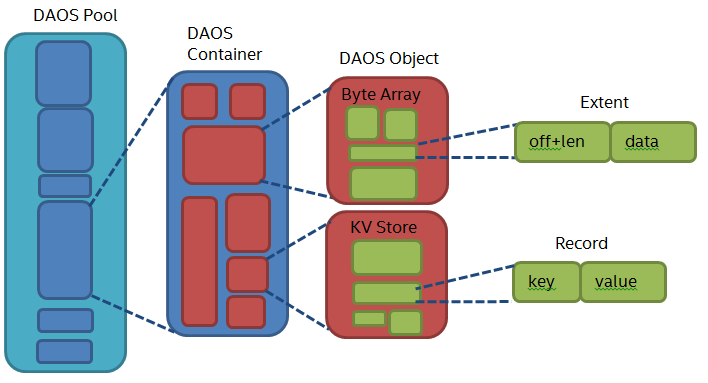
\includegraphics[width=\colwidth/2]{diagrams/DAOS_Pool_Cont_Obj.png}
      \caption{Diagram of DAOS pool data heirarchy.}
    \end{figure}
    
    DAOS can be accessed via the native DAOS library libdaos, mounting a container via DAOS FUSE, and the interception library libpil4dfs. 
    The native DAOS libary will provide the best performance, while the interception library provides the same perfromance for I/O operations without code changes.
    Metadata operations via dfuse are slower than using the DFS API as the DFS API bypasses the kernel entirely.

    \begin{figure}
      \centering
        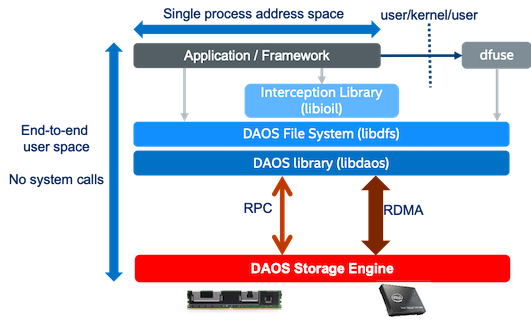
\includegraphics[width=\colwidth/2]{diagrams/posix.png}
      \caption{Diagram of DAOS storage system communication flow from applications to DAOS storage engines.}
    \end{figure}
    

  \end{block}

  \begin{block}{Aurora Architecture} 

    \begin{figure}
      \centering
        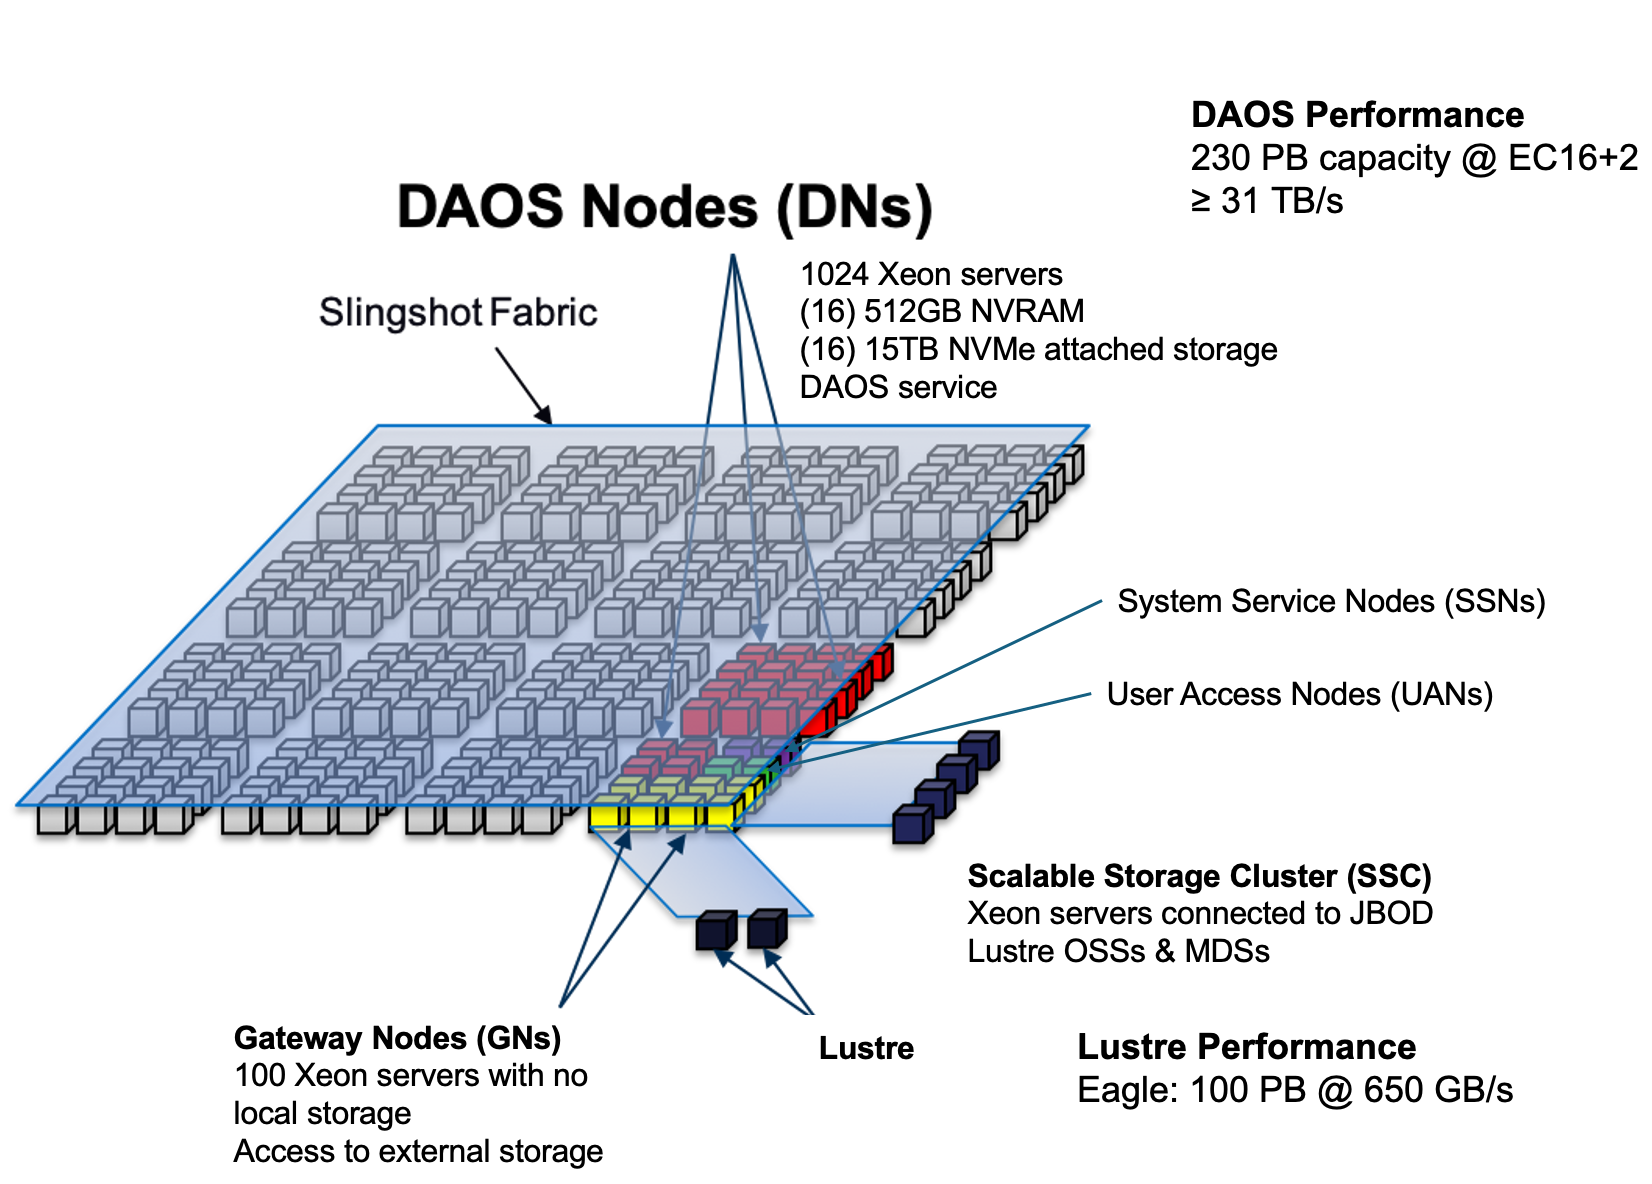
\includegraphics{diagrams/aurora-storage-architecture.png}
      \caption{Diagram of DAOS storage system architecture on Aurora from Argonne National Lab}
    \end{figure}

    Our pool had 127 nodes (4064 targets, 32 targets per node) with 3 TB Tier 0 (SCM) storage and 97 TB Tier 1 (NVMe) storage. Aurora compute nodes use two Intel Xeon CPU Max Series, with 52 cores each. For ior and mdtest we bind to 48 cores per node.
  \end{block}

  

% \begin{lstlisting}
% Pool 916ac7e2-bec3-4228-a065-b12ea9f4910e, ntarget=4064, disabled=0, 
% leader=140, version=1, state=Ready
% Pool health info:
% - Rebuild idle, 0 objs, 0 recs
% Pool space info:
% - Target(VOS) count:4064
% - Storage tier 0 (SCM):
%   Total size: 3.0 TB
%   Free: 2.7 TB, min:653 MB, max:655 MB, mean:654 MB
% - Storage tier 1 (NVMe):
%   Total size: 97 TB
%   Free: 97 TB, min:24 GB, max:24 GB, mean:24 GB

% \end{lstlisting}




\end{column}

\separatorcolumn

\begin{column}{\colwidth}


  \begin{block}{Benchmarking}
    We evaluated this storage system using the fio, ior, and mdtest I/O benchmarks.
    In particular we are interested on the effects of client-side scaling, 
    amount of data transferred at a time (block size for fio, transfer size for ior), 
    number of processes per node, and access type (read/write, random/sequential) 
    on latency, IOPS, and bandwidth.
    
  \end{block}

  \begin{block}{fio Bandwidth}

    
    
    \begin{figure}
      \centering
        \includesvg[width=\colwidth]{diagrams/fio_bw_vs_bs_hueRW_nj-16_iod-16.svg} 
      \caption{For one client node with 16 jobs with 16 I/O units kept in flight, the bandwidth vs block size for fio using the pvsync I/O engine. Block size in fio is the size of an I/O unit. This desmonstrates the performance achieved by POSIX container access via dfuse mount points. pvsync I/O engine uses vectorized system calls and allows read/write from non-contiguous buffers.}
    \end{figure}

    \begin{figure} 
      \centering
        \includesvg[width=\colwidth]{diagrams/bw_stacked_combined.svg} 
      % Read is reading only, 4:1 is 4 reads per write, 1:1 is an equal amount of reading and writing, 1:4 is 1 read per 4 writes, and write is writing only.
      \caption{For one client node with 16 jobs with 16 I/O units kept in flight, the proportions of overall bandwidth spent reading and writing across different workloads. The yellow line indicates the expected ratio of bandwidth proportions. Buffered I/O will use an intermediate buffer between applications (fio) and system calls to preadv*/pwritev*, while unbuffered I/O will go straight to system calls.}
    \end{figure}

    We did not observe a large difference in performance between random and sequential access patterns. 
    Additionally, for a dfuse access, changing the number of fio jobs (additional threads cloning the original thread) or I/O depth (number of I/O units to keep in flight) has little effect on performance.

  \end{block}

  \begin{block}{IOR Latency}
    \begin{figure} 
      \centering
        \includesvg[width=\colwidth]{diagrams/ior_latency.svg} 
      \caption{ For a transfer size of 1 MiB, the ior latency vs number of tasks. For <8 nodes, the write latency stays relatively constant as the number of tasks increases, but larger numbers of nodes accrue more latency as the number of tasks increases. Read latency ellicited a <10 ms increase in latency as more tasks were used, but all test cases stayed under 20 ms latency (10 ms difference from 1 task) except the largest number of nodes used (32). }
    \end{figure}
  \end{block}


\end{column}

\separatorcolumn

\begin{column}{\colwidth}

  \begin{block}{IOR Bandwidth}

    \begin{figure}
      \centering
        \includesvg[width=\colwidth]{diagrams/ior_bw-vs-tasks_hue-nodes-2M.svg} 
      \caption{For a transfer size of 2 MiB, the ior bandwidth vs number of tasks, using the DFS API}
    \end{figure}
    \begin{figure}
      \centering
        \includesvg[width=\colwidth]{diagrams/ior_bw-vs-tasks_hue-nodes_16M.svg} 
      \caption{For a transfer size of 16 MiB, the ior bandwidth vs number of tasks, using the DFS API.}
    \end{figure}
    With a large transfer size, we see that reading with more than 
    8 or 16 tasks per node decreases bandwidth dramatically, 
    although smaller numbers of tasks provide higher bandwidth 
    than the same number of tasks run with a smaller transfer size. 
    A small transfer size, such as 16 KiB provided relatively lower bandwidths 
    than either 1-2 MiB or 16 MiB, due to having to make many small I/O operations. 
    Reading has similar throughput to writing using the native DFS API, 
    until the number of nodes used become larger, when it surpassed write bandwidth.


    \begin{figure}
      \centering
        \includesvg[width=\dimexpr 3\colwidth/4\relax]{diagrams/ior_bw-vs-tx_8ppn.svg} 
      \caption{For a transfer size of 1 MiB, the ior bandwidth vs number of tasks, using the DFS API.}
    \end{figure}

    As with the pvsync I/O engine, 
    the DFS API begins to saturate at transfer sizes above 1-2 MiB. 
    The same transfer sizes, however, provide 2-3x higher bandwidth 
    for single-client workloads. Unlike the non-native API, 
    we see read bandwidths are on a similar scale to write bandwidth 
    and are higher overall, instead of being dramatically lower 
    than write bandwidths.
    
 
  \end{block}

  \begin{block}{Acknowledgments}
  This research used resources of the Argonne Leadership Computing Facility, which is a U.S. Department of Energy Office of Science User Facility operated under contract DE-AC02-06CH11357.
  \end{block}
  

  \begin{block}{References} 

    \nocite{*}
    \footnotesize{\bibliographystyle{plainnat}\bibliography{poster}}
 
  \end{block}

\end{column}

\separatorcolumn
\end{columns}
\end{frame}

\end{document}